\section{\texorpdfstring{$p$}{p} -adic numbers}

See \href{https://w3.math.cinvestav.mx/p-adic2019/sites/default/files/Zuniga.pdf}{Zuniga.pdf}

\begin{definition}[$p$-adic norm]
Let $p$ be a fixed prime number, and let $x$ be a nonzero rational number. Then, $x = p^k \frac{a}{b}$, with $p \nmid ab$, and $k \in \mathbb{Z}$. The \textbf{$p$-adic absolute value} (or \textbf{$p$-adic norm}) of $x$ is defined as
\[
|x|_p = \begin{cases} p^{-k} & \text{if } x \neq 0, \\ 0 & \text{if } x = 0. \end{cases}
\]
\end{definition}
\begin{definition}[non-Archimedean metric]
Let $(X,d)$ be a metric space. The metric $d$ is called \textbf{non-Archimedean} if
\[
d(x,y) \leq \max\left\{d\left(x,z\right),d\left(z,y\right)\right\} \text{ for any } x,y,z \in X.
\]
\end{definition}
\begin{exercise}
Let $\left(F,|\cdot|\right)$ be a valued field, where $|\cdot|$ is a non-Archimedean absolute value. Assume that $F$ is complete with respect to $|\cdot|$. Then, the series $\sum_{k \geq 0} a_k, a_k \in F$ converges if and only if $\lim_{k \to \infty} |a_k| = 0$.
\end{exercise}
\begin{theorem}[Ostrowski]
Any non trivial absolute value on $\mathbb{Q}$ is equivalent to $|\cdot|_p$ or to the standard absolute value $|\cdot|_\infty$.
\end{theorem}
\subsection{The field of \texorpdfstring{$p$}{p} -adic numbers}

\begin{lemma}
Consider the set
\[
\mathbb{Q}_p := \left\{ x = p^\gamma \sum_{i=0}^\infty x_i p^i : \gamma \in \mathbb{Z}, \ x_i \in \{0,1,\ldots,p-1\}, \ x_0 \neq 0 \right\} \cup \{0\}
\]
endowed with the p-adic norm $|\cdot|_p$. Then, the following assertions hold.
	\begin{enumerate}
		\item $(\mathbb{Q}_p, |\cdot|_p)$ is a complete metric space;
		\item $\mathbb{Q}$ is dense in $\mathbb{Q}_p$;
		\item $\mathbb{Q}_p$ is a field of characteristic zero;
		\item the completion of $(\mathbb{Q}, |\cdot|_p)$ is $(\mathbb{Q}_p, |\cdot|_p)$.
	\end{enumerate}
\end{lemma}
(i)
I don't understand.

(ii)
We set
\[
\mathbb{Z}_p:=\left\{x\in\mathbb{Q}_p:x=p^\gamma\sum_{i=0}^\infty x_ip^i;\gamma\in\mathbb{N},\:x_0\neq0\right\}.
\]
Then any $x\in \mathbb{Q}_{p}\setminus \{ 0 \}$ can be written as $x=p^{\gamma}\widetilde{x}$, with $\widetilde{x}\in \mathbb{Z}_{p}$ and $\lvert \widetilde{x} \rvert_{p}=1$. Given $p^{-L}$, $L>\gamma$, we have to show the existence of $\frac{a}{b}\in \mathbb{Q}$ such that $\left\lvert  x-\frac{a}{b}  \right\rvert_{p}<p^{-L}$. We take $b^{-1}=p^{\gamma}$ and $a\in \mathbb{Z}$ satisfying $\lvert a-\widetilde{x} \rvert_{p}<p^{-L+\gamma}$.

(iii) omitted

(iv) combine (i), (ii), (iii).

The field of $p$ -adic numbers $\mathbb{Q}_{p}$ is defined as the completion of $\mathbb{Q}$ w.r.t. the distance induced by $\lvert \cdot  \rvert_{p}$.

The unit ball
\[
\mathbb{Z}_{p}=\{ x\in \mathbb{Q}_{p}:\lvert x \rvert _{p}\leq 1 \}=\left\{  x\in \mathbb{Q}_{p} :x=\sum_{i=i_0}^{\infty} x_ip^{i},i_0\geq 0 \right\}
\]
is a PID. Any ideal of $\mathbb{Z}_{p}$ has the form
\[
p^{m}\mathbb{Z}_{p}=\left\{  x\in \mathbb{Z}_{p}:x=\sum_{i\geq m}^{} x_ip^{i}  \right\},\quad m\in \mathbb{N}
\]
Indeed, let $I\subseteq \mathbb{Z}_{p}$ be an ideal. Set $m_0=\min_{x\in I}\mathrm{ord}(x)\in \mathbb{N}$, and let $x_0\in I$ such that $\mathrm{ord}(x_0)=m_0$. Then $I=x_0\mathbb{Z}_{p}$.

From a geometric point of view, the ideals of the form $p^{m}\mathbb{Z}_{p}$, $m\in \mathbb{Z}$, constitute a fundamental system of neighborhoods around the origin in $\mathbb{Q}_{p}$.

The \textit{residue field} of $\mathbb{Q}_p$ is $\mathbb{Z}_p/p\mathbb{Z}_p \cong \mathbb{F}_p$ (the finite field with $p$ elements). The group of units of $\mathbb{Z}_p$ is
\[
\mathbb{Z}_p^{\times} = \{x \in \mathbb{Z}_p : |x|_p = 1\}.
\]

\begin{exercise}
$x=x_0+x_1p+\dots\in \mathbb{Z}_{p}$ is a unit iff $x_0\neq0$. Moreover if $x\in \mathbb{Q}_{p}\setminus \{ 0 \}$, then $x=p^{m}u$, $m\in \mathbb{Z}$, $u\in \mathbb{Z}_{p}^{\times}$.
\end{exercise}
\subsection{Topology of \texorpdfstring{$\mathbb{Q}_{p}$}{mathbbQ_p}}

Define
\[
B_{r}(a)=\{ x\in \mathbb{Q}_{p}:\lvert x-a \rvert _{p}\leq p^{r} \},r\in \mathbb{Z}
\]
as the ball with center $a$ and radius $p^{r}$, and
\[
S_{r}(a)=\{ x\in \mathbb{Q}_{p}:\lvert x-a \rvert _{p}=p^{r} \},r\in \mathbb{Z}
\]
as the sphere with center $a$ and radius $p^{r}$.

The radius are always integer powers of $p$.

\begin{remark}
Notice that $B_{r}(a)=a+p^{-r}\mathbb{Z}_{p}$ and $S_{r}(a)=a+p^{-r}\mathbb{Z}_{p}^{\times}$.
\end{remark}
We declare that the $B_{r}(a)$, $r\in \mathbb{Z}$, $a\in \mathbb{Q}_{p}$, are open subsets. These sets form a basis for the topology of $\mathbb{Q}_{p}$.

\begin{proposition}
$S_{r}(a)$, $B_{r}(a)$ are open and closed sets in the topology of $\mathbb{Q}_{p}$.
\end{proposition}
\begin{proof}
We first show that $S_{r}(a)$ is open. Notice that
\[
\begin{aligned}
S_{r}(a) & =a+p^{-r}\underbrace{ \mathbb{Z}_{p}^{\times} }_{ \underbrace{ x_0 }_{ \neq 0 }+x_1p+\dots\in } \\
 & =\bigsqcup_{x_0=1,2,\dots p-1}a+x_0p^{-r}+p^{-r+1}\underbrace{ \mathbb{Z}_{p} }_{ \sum_{i=i_0\geq 0}^{\infty}y_ip^{i}\in  } \\
 & =\bigsqcup _{i\in \{ 1,\dots,p-1 \}}\underbrace{ B_{(r-1)}(a+p^{-r}i) }_{ \text{open} } 
\end{aligned}
\]
Consequently, $S_{r}(a)$ is open.

\begin{figure}[H]
\centering
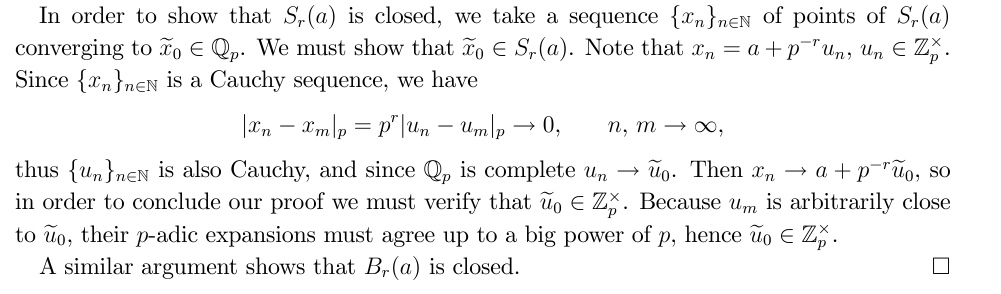
\includegraphics[width=\textwidth]{p-adic-2025051522.png}
% \caption{}
\label{}
\end{figure}

\end{proof}

\begin{lemma}
If $b \in B_r(a)$ then $B_r(b) = B_r(a)$, i.e. any point of the ball $B_r(a)$ is its center.
\end{lemma}
\begin{proof}
Let $x \in B_r(b)$, then
\[
|x - a|_p = |x - b + b - a|_p \leq \max \{ |x - b|_p, |b - a|_p \} \leq p^r,
\]
i.e. $B_r(b) \subseteq B_r(a)$.

Since $a \in B_r(b)$ (i.e. $|b - a|_p = |a - b|_p \leq p^r$), we can repeat the previous argument to show that $B_r(a) \subseteq B_r(b)$.
\end{proof}

\begin{exercise}
Any two balls in $\mathbb{Q}_{p}$ are either disjoint or one is contained in another.
\end{exercise}
\begin{exercise}
The boundary of any ball is the empty set.
\end{exercise}
\begin{theorem}
A set $K\subset \mathbb{Q}_{p}$ is compact iff closed and bounded.
\end{theorem}
\subsection{The \texorpdfstring{$n$}{n} -dimensional \texorpdfstring{$p$}{p} -adic space}

We extend the $p$ -adic norm to $\mathbb{Q}_{p}^{n}$ by taking
\[
\lVert x \rVert _{p}\coloneqq \max_{1\leq i\leq d}\lvert x_i \rvert _{p},\text{ for }x=(x_1,\dots,x_n)\in \mathbb{Q}^{n}_{p}
\]
We define $\mathrm{ord}(x)=\min_{1\leq i\leq n}\{ \mathrm{ord}(x_i) \}$, then $\lVert x \rVert_{p}=p^{-\mathrm{ord}(x)}$.
\[
B_{r}^{n}(a)=\{ x\in \mathbb{Q}^{n}_{p}:\lVert x-a \rVert _{p}\leq p^{r} \}=B_{r}(a_1)\times \dots \times B_{r}(a_{n})
\]
\[
S_{r}^{n}(a)=\{ x\in \mathbb{Q}_{p}^{n}:\lVert x-a \rVert _{p}=p^{r} \}
\]
Note that $S^{1}_{0}=\mathbb{Z}_{p}^{\times}$ but $(\mathbb{Z}_{p}^{\times})^{n}\subsetneq S_0^{n}$.

As a topological space $(\mathbb{Q}_{p}^{n},\lVert \cdot  \rVert_{p})$ is totally disconnected, i.e. the only connected subsets of $\mathbb{Q}^{n}_{p}$ are the empty set and the points.

\subsection{Exercises}

\begin{exercise}[yau-2020-problem-5]
\begin{figure}[H]
\centering
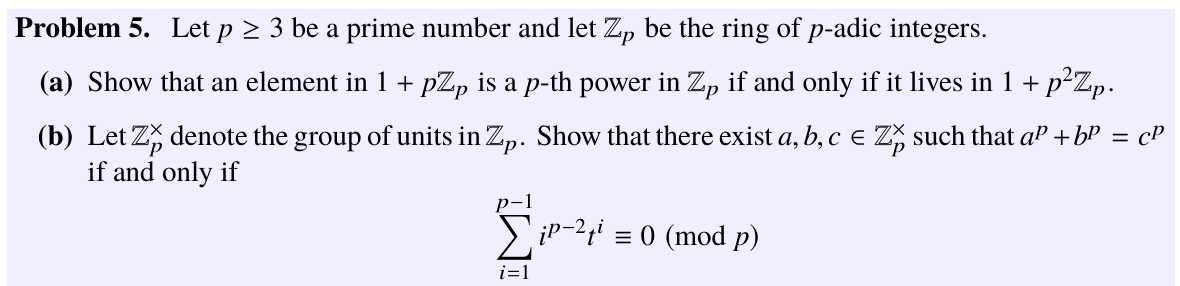
\includegraphics[width=\textwidth]{p-adic-2025051523.png}
% \caption{}
\label{}
\end{figure}
\begin{figure}[H]
\centering
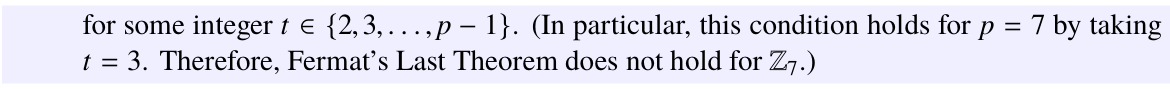
\includegraphics[width=\textwidth]{1-p-adic-2025051523.png}
% \caption{}
\label{}
\end{figure}
\end{exercise}
\begin{figure}[H]
\centering
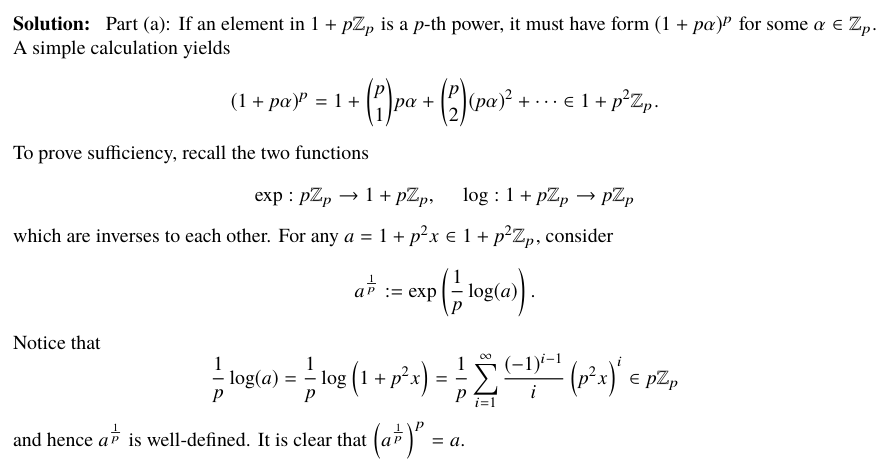
\includegraphics[width=\textwidth]{3-p-adic-2025051523.png}
% \caption{}
\label{}
\end{figure}
\begin{figure}[H]
\centering
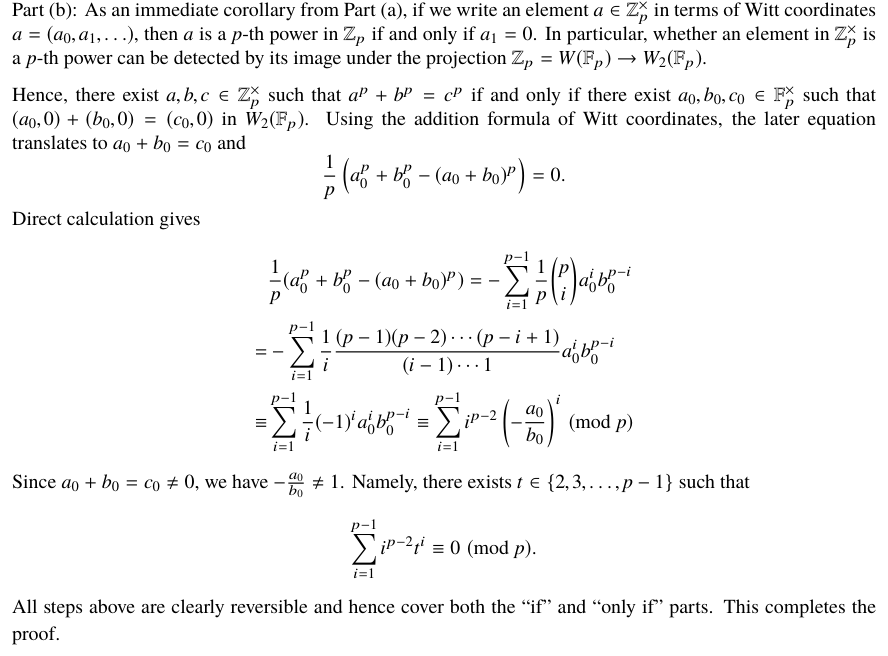
\includegraphics[width=\textwidth]{4-p-adic-2025051523.png}
% \caption{}
\label{}
\end{figure}
